\chapter{Risultati}
\label{section:results}

\section{Rilevamento dei volti}
\label{section:results_fd}

Nel rilevamento dei volti la combinazione dei due modelli pretrainati mostra
una percentuale di rilevamento molto alta, quasi al 100\% nel caso in cui i volti sono 
fotografati frontalmente; i risultati peggiorano invece se il volto è girato oppure 
inquadrato solo in parte. 

\smallskip

\begin{figure}[h]
    \centering
    \begin{subfigure}[b]{0.7\linewidth}
      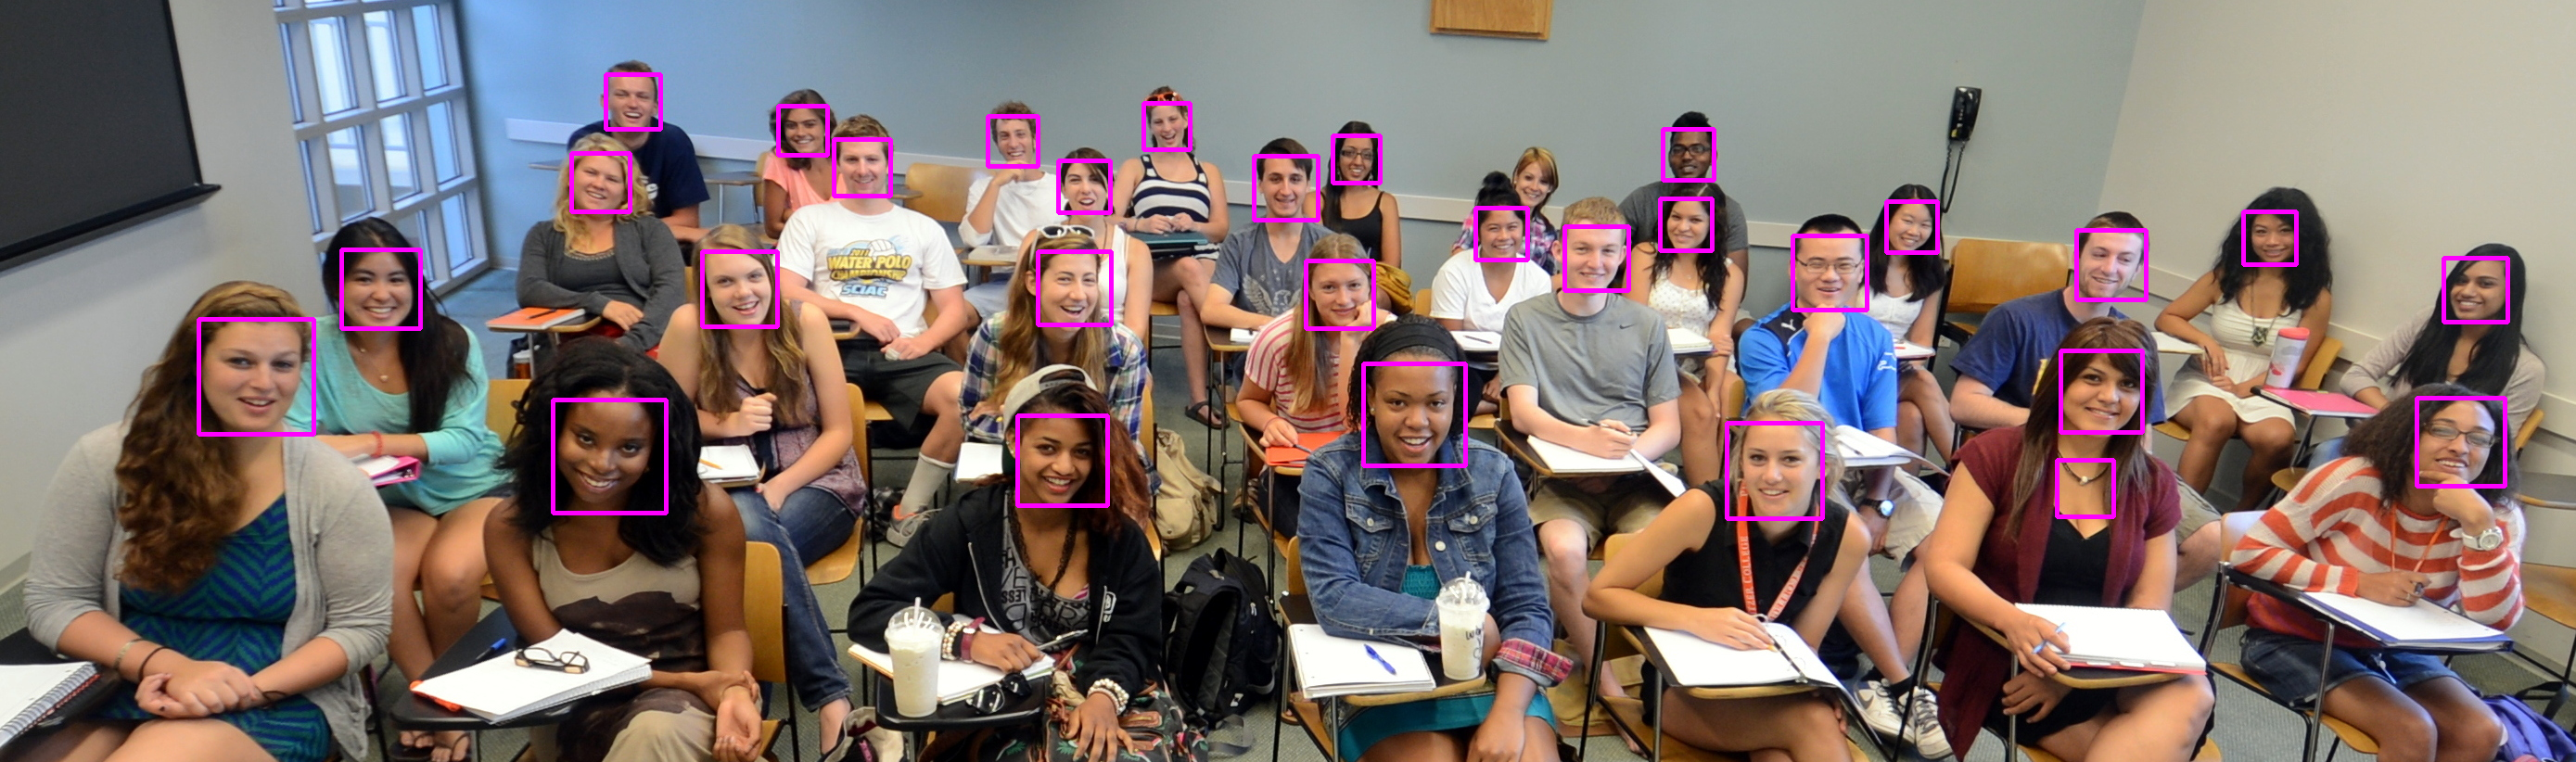
\includegraphics[width=\linewidth]{detected_3.png}
    \end{subfigure}

    \smallskip
    
    \begin{subfigure}[b]{0.7\linewidth}
        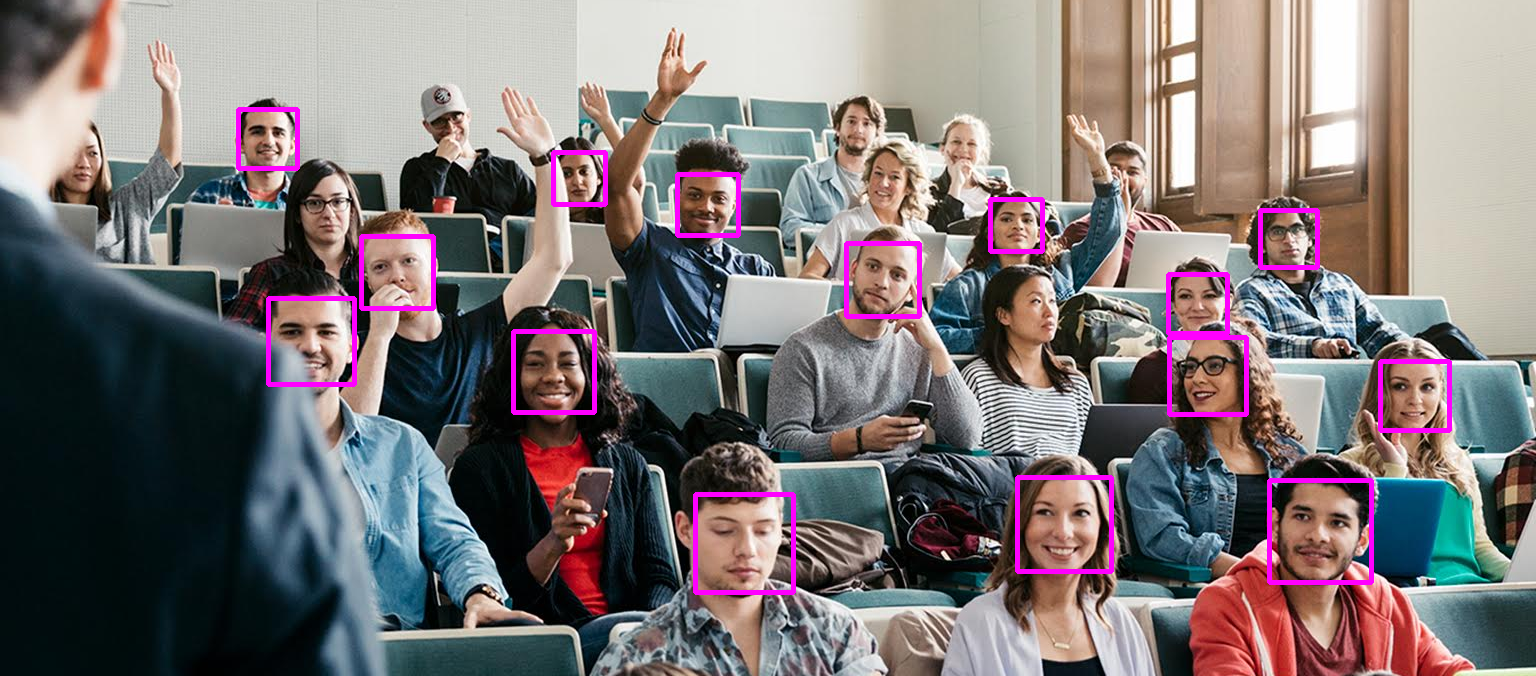
\includegraphics[width=\linewidth]{detected_1.png}
    \end{subfigure}

    \smallskip
    
    \begin{subfigure}[b]{0.7\linewidth}
        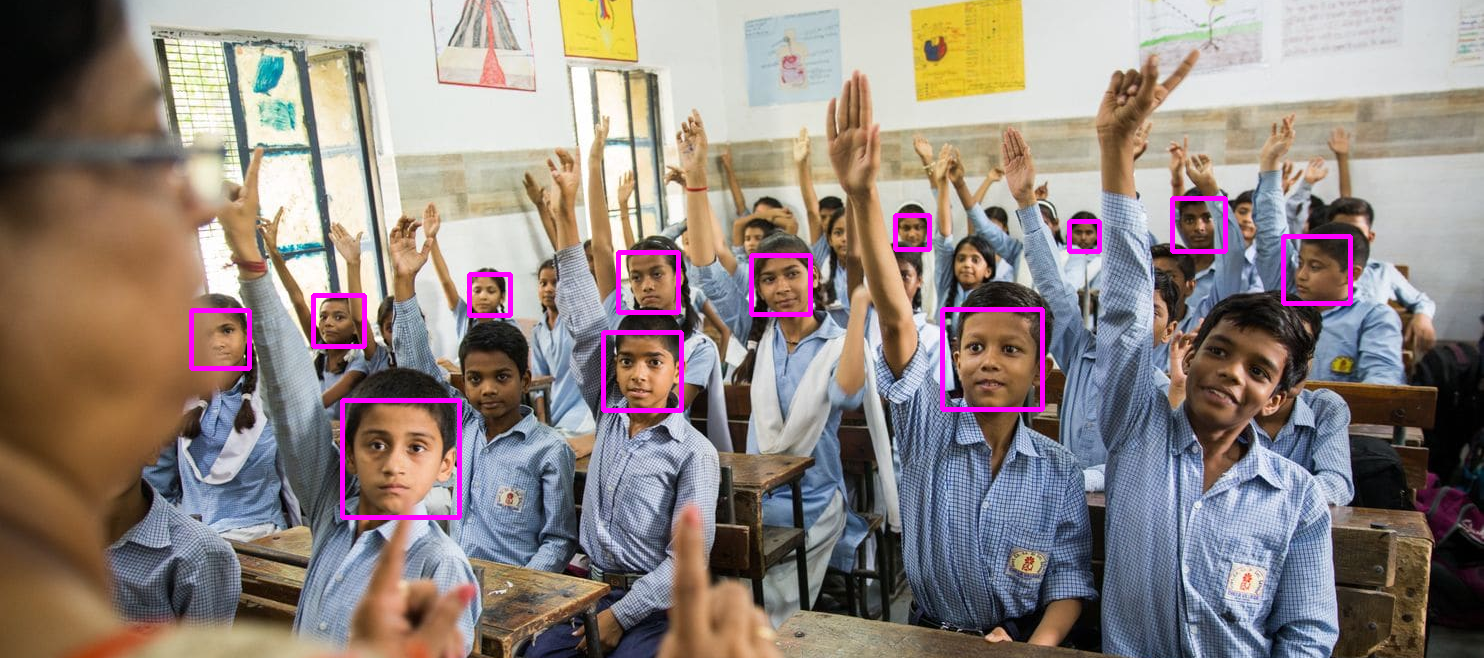
\includegraphics[width=\linewidth]{detected_2.png}
    \end{subfigure}
    \caption{Esempi di face detection su immagini di aule con studenti}
    \label{fig:example_opencv}
\end{figure}

\section{Rendimento della rete}
\label{section:results_ml}

Il dataset utilizzato contiene 1000 entry, ed il training, a causa dell'
\textit{early stopping} si ferma intorno alla 50 esima iterazione con i seguenti 
score sul set di \textit{test}

\smallskip

\begin{figure}[h]
    \centering
    
    \begin{subfigure}[b]{0.45\linewidth}
        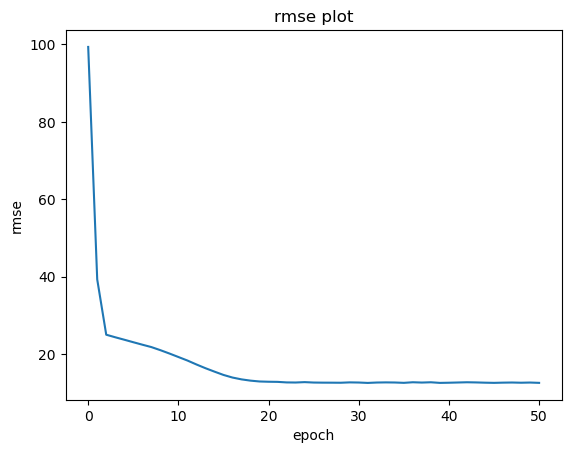
\includegraphics[width=\linewidth]{plots/rmse.png}
        \caption{RMSE}
    \end{subfigure}
    \begin{subfigure}[b]{0.45\linewidth}
        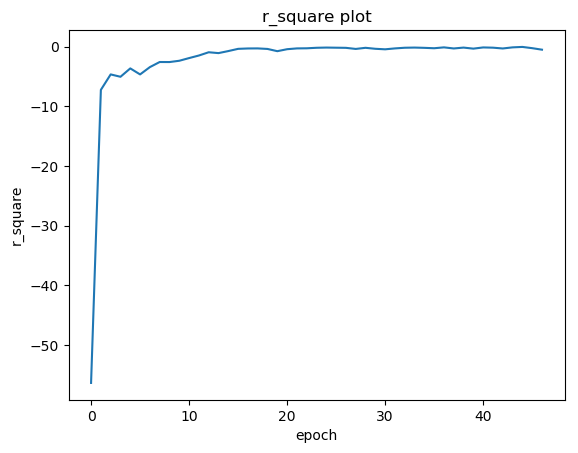
\includegraphics[width=\linewidth]{plots/r_square.png}
        \caption{$r^2$}
    \end{subfigure}
    \begin{subfigure}[b]{0.9\linewidth}
        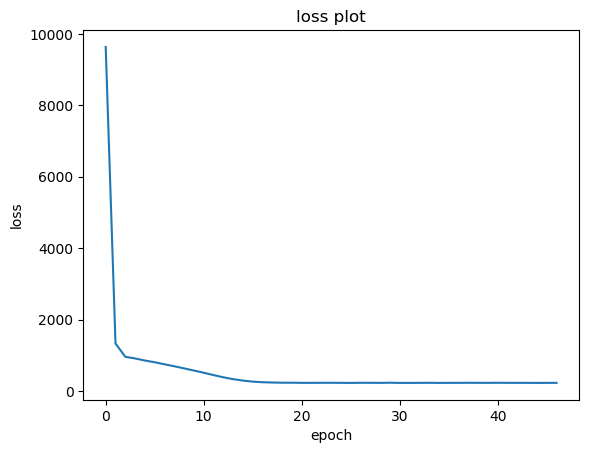
\includegraphics[width=\linewidth]{plots/loss.png}
        \caption{MSE}
    \end{subfigure}
    \caption{Gli score della rete}
    \label{fig:example_opencv}
\end{figure}

\newpage

\section{Allocazione nelle aule}
\label{section:results_mp}

Avendo fornito come test il seguente set di aule

\begin{table}[h]
    \begin{small}
        \begin{center}
            \begin{tabular}[c]{c|c}
                Nome aula & Capacità \\
                \hline
                r00 & 40 \\
                r01 & 50 \\
                r02 & 60 \\
                r03 & 70 \\
                r04 & 80 \\
                r05 & 90 \\
                r06 & 100 \\
                r07 & 110 \\
                r08 & 120 \\
                r09 & 130 
            \end{tabular}
        \end{center}
    \end{small}
\end{table}

\noindent
i problemi proposti vengono risolti con i seguenti assegnamenti

\begin{table}[h]
    \begin{small}
        \begin{center}
            \begin{tabular}[c]{c|c|c|c|c}
                Giorno & Ora & Disciplina & Stima studenti & Aula assegnata \\
                \hline
                sunday & 15 & SC2 & 86 & r05 \\
                sunday & 15 & PSW & 90 & r06 \\
                sunday & 15 & PFP & 115 & r08 \\
                monday & 10 & SC2 & 84 & r05
            \end{tabular}
        \end{center}
    \end{small}
\end{table}

\section{Analisi dei risultati}

I risultati ottenuti sono considerabili molto positivi:

\begin{itemize}
    \item In \textbf{\nameref{section:results_fd}} si nota come anche solo con due modelli pretrainati
        computazionalmente poco onerosi si sia raggiunto un rilevamento quasi totale dei volti
    \item In \textbf{\nameref{section:results_ml}} gli score, ottenuti da una rete neurale molto semplice,
        evidenziano, in particolare il RMSE, come l'errore nelle stime effettuate sia circa 
        di 5 studenti, circa il 5\% del numero medio di studenti del dataset
    \item In \textbf{\nameref{section:results_mp}} gli assegnamenti effettuati dall'applicazione rispettano
        completamente le richieste precedentemente specificate.
\end{itemize}
